\documentclass[a4paper, 11pt]{article}

\usepackage{graphicx}
\usepackage{setspace}
\usepackage{fontspec}
\usepackage{float}
\usepackage{enumitem}
\usepackage{caption}
\usepackage{url}
\usepackage{tikz}
\usetikzlibrary{shapes.geometric, arrows.meta, positioning, calc, fit, backgrounds}
\usepackage{booktabs}
\usepackage{tabularx}
\usepackage{makecell}
\usepackage{multirow}
\usepackage[table]{xcolor}
\usepackage{amsmath}
\usepackage{amssymb}
\usepackage[margin=2.0cm, top=2.2cm, bottom=2.2cm]{geometry}
\usepackage{tcolorbox}
\usepackage{fancyhdr}
\usepackage{hyperref}
\usepackage{listings}

\setmainfont{Times New Roman}
\setmonofont[Scale=0.85]{Courier New}

\hypersetup{
    colorlinks=true,
    linkcolor=blue!70!black,
    citecolor=blue!70!black,
    urlcolor=blue!70!black,
    pdfborder={0 0 0}
}

\pagestyle{fancy}
\fancyhf{}
\rhead{\small\textit{Cambodia CPI Pipeline: Data Lineage \& Column Dictionary}}
\lhead{\small\textit{Enterprise Data Governance \& Technical Specification}}
\rfoot{\small Page \thepage}
\renewcommand{\headrulewidth}{0.4pt}
\renewcommand{\footrulewidth}{0.4pt}

\definecolor{cambodiablue}{RGB}{24, 64, 118}
\definecolor{cambodiared}{RGB}{198, 12, 48}
\definecolor{primaryblue}{RGB}{24, 64, 118}
\definecolor{secondaryblue}{RGB}{41, 128, 185}
\definecolor{lightbg}{RGB}{245, 248, 252}
\definecolor{accentgreen}{RGB}{39, 174, 96}
\definecolor{boxgray}{RGB}{248, 249, 250}
\definecolor{goldorange}{RGB}{211, 84, 0}
\definecolor{silvergray}{RGB}{127, 140, 141}
\definecolor{bronzebr}{RGB}{160, 82, 45}

\tcbset{
    sharp corners,
    colback=lightbg,
    colframe=primaryblue,
    boxrule=1pt,
    fonttitle=\bfseries,
    coltitle=white
}

\lstset{
    basicstyle=\ttfamily\small,
    breaklines=true,
    backgroundcolor=\color{boxgray},
    frame=single,
    rulecolor=\color{gray!30},
    keywordstyle=\color{primaryblue}\bfseries,
    commentstyle=\color{gray},
    stringstyle=\color{cambodiared}
}

\title{\vspace{-1.2cm}
\begin{tcolorbox}[colback=primaryblue, colframe=primaryblue, arc=2mm]
\centering \color{white}
{\Huge \textbf{Cambodia Daily Consumer Price Index (CPI)}}\\[6pt]
{\Large End-to-End Data Lineage, Transformation Logic, and Column Dictionary}\\[4pt]
{\large Medallion Architecture Specification (Bronze $\to$ Silver $\to$ Gold $\to$ Econometric Nowcast)}
\end{tcolorbox}
\vspace{-0.5cm}}

\author{\textbf{National Institute of Statistics (NIS) \& National Bank of Cambodia (NBC) Research Collaboration}\\[2pt]
\small High-Frequency Economic Nowcasting Laboratory $\cdot$ Big Data Econometrics Engineering Unit}
\date{\small Version 3.4 -- September 21, 2026}

\begin{document}

\maketitle

\begin{abstract}
\noindent This technical specification provides the complete, auditable end-to-end data lineage, transformation mathematics, and column-level dictionary for the \textbf{Cambodia Daily Consumer Price Index (CPI) Medallion Data Platform}. The platform daily ingests multi-source unstructured and semi-structured retail data across 25 retail web scrapers and official government APIs, processing over 120,000 raw daily product observations into conformed UN COICOP 2018 analytical marts and econometric nowcasts. This document rigorously traces every table and column across the Medallion progression: from raw JSON extraction in \textbf{Bronze (Staging)}, through text normalization, vector cosine deduplication, and AI classification in \textbf{Silver}, up to Jevons micro-indices, Laspeyres macro synthesis, and 5-basket RidgeCV nowcasting in \textbf{Gold}. Each column is formally mapped with its source provenance, SQL transformation expression, mathematical formula, nullability constraint, and business definition.
\end{abstract}

\vspace{0.3cm}
\tableofcontents
\newpage

% =============================================================================
\section{Medallion Architectural Lineage Overview}
% =============================================================================

The Cambodia CPI data platform is architectured as a strict Medallion data engineering pipeline operating on a single-writer, dependency-enforced DAG topology managed by Apache Airflow 2.9.3 and dbt Core. 

\begin{figure}[H]
\centering
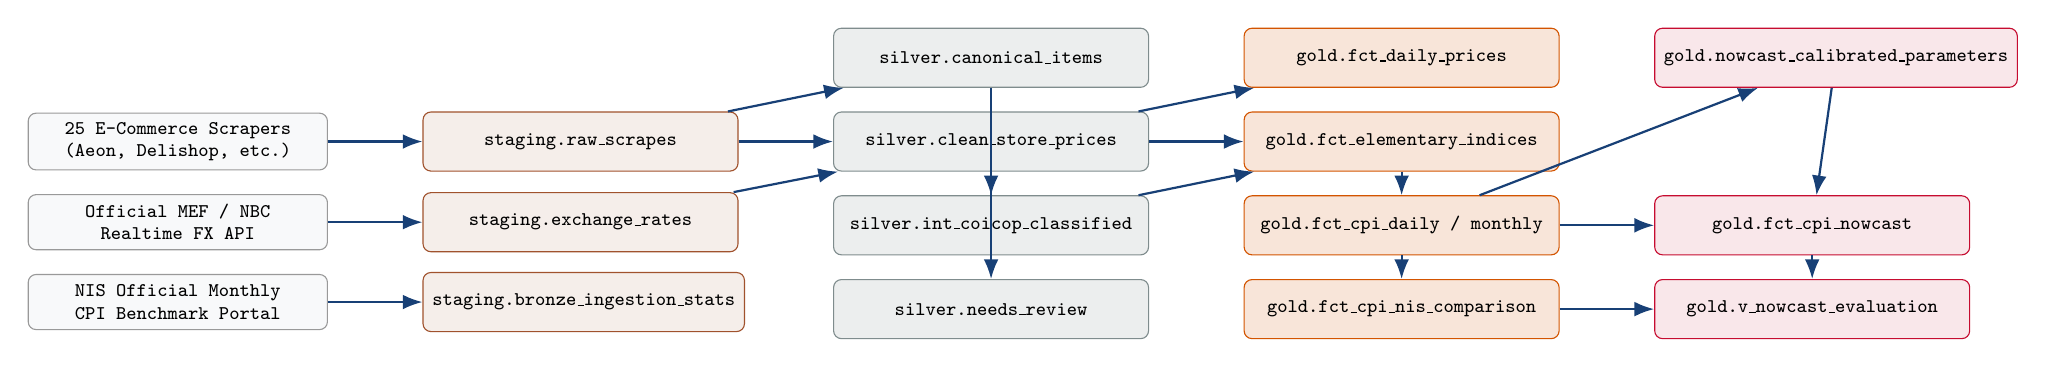
\begin{tikzpicture}[
    node distance=1.3cm and 0.8cm,
    layerbox/.style={draw=primaryblue!80, fill=white, rounded corners=3mm, thick, inner sep=6pt, font=\small},
    tablebox/.style={draw=gray!80, fill=boxgray, rounded corners=1mm, font=\scriptsize\ttfamily, minimum width=3.8cm, minimum height=0.7cm, align=center},
    bronzebox/.style={draw=bronzebr, fill=bronzebr!10, rounded corners=1mm, font=\scriptsize\ttfamily\bfseries, minimum width=4.0cm, minimum height=0.75cm, align=center},
    silverbox/.style={draw=silvergray, fill=silvergray!15, rounded corners=1mm, font=\scriptsize\ttfamily\bfseries, minimum width=4.0cm, minimum height=0.75cm, align=center},
    goldbox/.style={draw=goldorange, fill=goldorange!15, rounded corners=1mm, font=\scriptsize\ttfamily\bfseries, minimum width=4.0cm, minimum height=0.75cm, align=center},
    mlbox/.style={draw=cambodiared, fill=cambodiared!10, rounded corners=1mm, font=\scriptsize\ttfamily\bfseries, minimum width=4.0cm, minimum height=0.75cm, align=center},
    arrow/.style={-{Latex[length=2.5mm]}, thick, primaryblue}
]

% Ingestion Sources
\node (src1) [tablebox] {25 E-Commerce Scrapers\\(Aeon, Delishop, etc.)};
\node (src2) [tablebox, below=0.3cm of src1] {Official MEF / NBC\\Realtime FX API};
\node (src3) [tablebox, below=0.3cm of src2] {NIS Official Monthly\\CPI Benchmark Portal};

% Bronze Layer
\node (b_raw) [bronzebox, right=1.2cm of src1] {staging.raw\_scrapes};
\node (b_fx) [bronzebox, right=1.2cm of src2] {staging.exchange\_rates};
\node (b_stats) [bronzebox, right=1.2cm of src3] {staging.bronze\_ingestion\_stats};

% Silver Layer
\node (s_clean) [silverbox, right=1.2cm of b_raw] {silver.clean\_store\_prices};
\node (s_items) [silverbox, above=0.3cm of s_clean] {silver.canonical\_items};
\node (s_coicop) [silverbox, below=0.3cm of s_clean] {silver.int\_coicop\_classified};
\node (s_review) [silverbox, below=0.3cm of s_coicop] {silver.needs\_review};

% Gold Layer
\node (g_fact) [goldbox, right=1.2cm of s_items] {gold.fct\_daily\_prices};
\node (g_micro) [goldbox, right=1.2cm of s_clean] {gold.fct\_elementary\_indices};
\node (g_macro) [goldbox, right=1.2cm of s_coicop] {gold.fct\_cpi\_daily / monthly};
\node (g_nis) [goldbox, right=1.2cm of s_review] {gold.fct\_cpi\_nis\_comparison};

% ML Layer
\node (ml_calib) [mlbox, right=1.2cm of g_fact] {gold.nowcast\_calibrated\_parameters};
\node (ml_now) [mlbox, right=1.2cm of g_macro] {gold.fct\_cpi\_nowcast};
\node (ml_eval) [mlbox, right=1.2cm of g_nis] {gold.v\_nowcast\_evaluation};

% Arrows
\draw [arrow] (src1) -- (b_raw);
\draw [arrow] (src2) -- (b_fx);
\draw [arrow] (src3) -- (b_stats);

\draw [arrow] (b_raw) -- (s_items);
\draw [arrow] (b_raw) -- (s_clean);
\draw [arrow] (b_fx) -- (s_clean);
\draw [arrow] (s_items) -- (s_coicop);
\draw [arrow] (s_items) -- (s_review);

\draw [arrow] (s_clean) -- (g_fact);
\draw [arrow] (s_clean) -- (g_micro);
\draw [arrow] (s_coicop) -- (g_micro);
\draw [arrow] (g_micro) -- (g_macro);
\draw [arrow] (g_macro) -- (g_nis);

\draw [arrow] (g_macro) -- (ml_calib);
\draw [arrow] (g_macro) -- (ml_now);
\draw [arrow] (ml_calib) -- (ml_now);
\draw [arrow] (ml_now) -- (ml_eval);
\draw [arrow] (g_nis) -- (ml_eval);

\end{tikzpicture}
\caption{Complete End-to-End DAG Data Flow: From Raw Retail Sources to Analytical Fact Marts and Econometric Nowcasts.}
\end{figure}

\subsection{Pipeline Execution Cadence \& Single-Writer Architecture}
Data flows sequentially across four Airflow DAGs executing on an ICT daily schedule:
\begin{enumerate}[leftmargin=*]
    \item \textbf{Scraper Ingestion Fan-Out (02:00--05:30 ICT)}: 25 asynchronous Python scrapers extract raw listings and land JSON batches into \texttt{staging.raw\_scrapes}.
    \item \textbf{Ingestion Circuit Breaker (05:45 ICT)}: \texttt{pipeline/circuit\_breaker.py} evaluates price velocity deltas against 7-day rolling medians. Anomalous batches are quarantined in \texttt{ops.circuit\_breaker\_events}.
    \item \textbf{Silver Curation DAG (06:00 ICT)}: Normalizes strings, assigns 768-dimensional embeddings via Gemini, runs pgvector cosine clustering, executes 5-tier COICOP classification, and unifies dual-currency prices into KHR.
    \item \textbf{Gold Synthesis \& Nowcasting DAG (08:00 ICT)}: Computes axiomatic Jevons micro-indices, aggregates Laspeyres 12-division indices, estimates expanding RidgeCV parameters, and executes the intra-month discrete arithmetic mean nowcast.
\end{enumerate}

\newpage
% =============================================================================
\section{Bronze Staging Layer: Ingestion \& Circuit Breakers}
% =============================================================================

\subsection{Table: \texttt{staging.raw\_scrapes}}
\textbf{Description}: Append-only raw landing table storing immutable batch payloads from scrapers. \\
\textbf{Grain}: One row per scrape execution batch per store. \\
\textbf{Authoritative Writer}: \texttt{pipeline/bronze\_ingestion.py}.

\begin{table}[H]
\centering
\small
\begin{tabularx}{\textwidth}{l p{2.8cm} c c p{4.0cm} X}
\toprule
\textbf{Target Column} & \textbf{Data Type} & \textbf{PK} & \textbf{Null?} & \textbf{Source Column / Expr} & \textbf{Business Definition \& Logic} \\
\midrule
\texttt{scrape\_id} & \texttt{UUID} & $\checkmark$ & No & \texttt{uuid.uuid4()} & Deterministic primary surrogate key for the scrape execution batch. \\
\texttt{store\_slug} & \texttt{VARCHAR(50)} & & No & Scraper metadata identifier & Unique identifier of the retail source (e.g. \texttt{'aeon'}, \texttt{'delishop'}). \\
\texttt{scrape\_date} & \texttt{DATE} & & No & Current date in Asia/Phnom\_Penh & Accounting date for price validity. \\
\texttt{payload} & \texttt{JSONB} & & No & HTTP / Browser JSON Array & Raw unparsed array of product dictionaries containing title, price, etc. \\
\texttt{record\_count} & \texttt{INTEGER} & & No & \texttt{len(payload)} & Total items harvested in this batch. \\
\texttt{created\_at} & \texttt{TIMESTAMPTZ} & & No & \texttt{NOW() AT TIME ZONE 'UTC'} & Immutable UTC ingestion timestamp. \\
\bottomrule
\end{tabularx}
\caption{Detailed Column Lineage for \texttt{staging.raw\_scrapes}.}
\end{table}

\subsection{Table: \texttt{staging.exchange\_rates}}
\textbf{Description}: Daily official USD/KHR exchange rates for dual-currency normalization. \\
\textbf{Grain}: One row per calendar date. \\
\textbf{Authoritative Writer}: \texttt{pipeline/mef\_fx\_importer.py}.

\begin{table}[H]
\centering
\small
\begin{tabularx}{\textwidth}{l p{2.8cm} c c p{4.0cm} X}
\toprule
\textbf{Target Column} & \textbf{Data Type} & \textbf{PK} & \textbf{Null?} & \textbf{Source Column / Expr} & \textbf{Business Definition \& Logic} \\
\midrule
\texttt{execution\_date} & \texttt{DATE} & $\checkmark$ & No & MEF API response \texttt{date} & Official publication date of the exchange rate. \\
\texttt{rate} & \texttt{NUMERIC(10,4)} & & No & MEF \texttt{rate} (fallback: NBC/4044) & Khmer Riel (KHR) per 1.00 USD. Clamped to $[3800, 4500]$. \\
\texttt{source\_currency} & \texttt{VARCHAR(3)} & & No & Constant \texttt{'USD'} & Base quotation currency. \\
\texttt{target\_currency} & \texttt{VARCHAR(3)} & & No & Constant \texttt{'KHR'} & Local transaction settlement currency. \\
\texttt{source\_api} & \texttt{VARCHAR(50)} & & No & Provider identifier & Provenance tag (\texttt{'mef\_api'}, \texttt{'nbc\_api'}, \texttt{'fallback\_static'}). \\
\texttt{fetched\_at} & \texttt{TIMESTAMPTZ} & & No & \texttt{NOW()} & Audit timestamp of API extraction. \\
\bottomrule
\end{tabularx}
\caption{Detailed Column Lineage for \texttt{staging.exchange\_rates}.}
\end{table}

\subsection{Table: \texttt{ops.circuit\_breaker\_events}}
\textbf{Description}: Automated security barrier logs preventing corrupt ingestion batches from entering Silver. \\
\textbf{Grain}: One row per evaluated store ingestion batch. \\
\textbf{Authoritative Writer}: \texttt{pipeline/circuit\_breaker.py}.

\begin{table}[H]
\centering
\small
\begin{tabularx}{\textwidth}{l p{2.5cm} c c p{4.0cm} X}
\toprule
\textbf{Target Column} & \textbf{Data Type} & \textbf{PK} & \textbf{Null?} & \textbf{Source Column / Expr} & \textbf{Business Definition \& Logic} \\
\midrule
\texttt{event\_id} & \texttt{BIGSERIAL} & $\checkmark$ & No & Database sequence & Unique auto-incrementing audit log identifier. \\
\texttt{store\_slug} & \texttt{VARCHAR(50)} & & No & \texttt{raw\_scrapes.store\_slug} & Retailer under evaluation. \\
\texttt{scrape\_date} & \texttt{DATE} & & No & \texttt{raw\_scrapes.scrape\_date} & Date under evaluation. \\
\texttt{status} & \texttt{VARCHAR(20)} & & No & Evaluated decision & Gate outcome: \texttt{'PASSED'}, \texttt{'WARNING\_FLAGGED'}, or \texttt{'HALTED'}. \\
\texttt{record\_count} & \texttt{INTEGER} & & No & Batch record count & Number of observations in batch. \\
\texttt{median\_price\_khr} & \texttt{NUMERIC(12,2)} & & No & Batch median price & Current day median item price normalized to KHR. \\
\texttt{price\_velocity\_delta\_pct} & \texttt{NUMERIC(6,2)} & & Yes & $\frac{\text{Med}_t - \text{Med}_{7d}}{\text{Med}_{7d}} \times 100\%$ & Percentage drift from rolling 7-day median. Flags warning if $>15\%$. \\
\texttt{created\_at} & \texttt{TIMESTAMPTZ} & & No & \texttt{NOW()} & Evaluation timestamp. \\
\bottomrule
\end{tabularx}
\caption{Detailed Column Lineage for \texttt{ops.circuit\_breaker\_events}.}
\end{table}

\newpage
% =============================================================================
\section{Silver Layer: Normalization, Embeddings \& Classification}
% =============================================================================

\subsection{Table: \texttt{silver.canonical\_items}}
\textbf{Description}: Central product catalog deduplicating distinct store listings into unified representative varieties. \\
\textbf{Grain}: One row per unique canonical consumer product. \\
\textbf{Authoritative Writer}: \texttt{pipeline/canonical\_matcher.py}.

\begin{table}[H]
\centering
\small
\begin{tabularx}{\textwidth}{l p{2.5cm} c c p{4.2cm} X}
\toprule
\textbf{Target Column} & \textbf{Data Type} & \textbf{PK} & \textbf{Null?} & \textbf{Source Column / Expr} & \textbf{Business Definition \& Logic} \\
\midrule
\texttt{item\_id} & \texttt{UUID} & $\checkmark$ & No & \texttt{uuid5(DNS, clean\_name)} & Master product surrogate key. \\
\texttt{canonical\_name} & \texttt{TEXT} & & No & Cleaned string from \texttt{pipeline/text\_clean.py} & Deterministically normalized product name: uppercase, stripped of promo noise and diacritics. \\
\texttt{brand} & \texttt{VARCHAR(100)} & & Yes & Regex extraction / payload & Identified brand entity (e.g. \texttt{'COCA COLA'}, \texttt{'NESTLE'}). \\
\texttt{package\_size} & \texttt{TEXT} & & Yes & Regex extraction & Raw normalized size descriptor (e.g. \texttt{'500g'}, \texttt{'1L'}). \\
\texttt{unit\_value} & \texttt{NUMERIC(10,3)} & & Yes & Numerical regex parse & Standardized quantity magnitude (e.g. \texttt{500.0}). \\
\texttt{unit\_metric} & \texttt{VARCHAR(10)} & & Yes & Unit extraction regex & Standardized measurement metric (\texttt{'g'}, \texttt{'kg'}, \texttt{'ml'}, \texttt{'l'}). \\
\texttt{match\_method} & \texttt{VARCHAR(30)} & & No & Resolution engine tag & Discovery lineage: \texttt{'exact\_match'}, \texttt{'embedding\_similarity'}, or \texttt{'new\_item'}. \\
\texttt{match\_confidence} & \texttt{NUMERIC(5,4)} & & No & Cosine score: $1 - \text{dist}$ & Vector match similarity score $\in [0.0000, 1.0000]$. Threshold $\ge 0.8500$. \\
\texttt{created\_at} & \texttt{TIMESTAMPTZ} & & No & \texttt{NOW()} & Item registration timestamp. \\
\bottomrule
\end{tabularx}
\caption{Detailed Column Lineage for \texttt{silver.canonical\_items}.}
\end{table}

\subsection{Hierarchical Precedence: \texttt{silver.int\_coicop\_classified}}
\textbf{Description}: Intermediate dbt transformation resolving UN COICOP 2018 classification codes. \\
\textbf{Transformation Macro}: \texttt{dbt/macros/coicop\_classify\_macro.sql}.

\begin{tcolorbox}[title=5-Tier Classification Resolution Precedence]
The COICOP code for an item is resolved via a strict SQL \texttt{CASE} precedence cascade:
\begin{enumerate}[leftmargin=*]
    \item \textbf{Tier 1: Exact Overrides (\texttt{coicop\_override.csv})}: Deterministic overrides for verified ambiguous products.
    \item \textbf{Tier 2: Store Purity Mapping}: Mono-category stores mapped directly (e.g. PPWSA $\to$ Division 04 Water, EDC $\to$ Division 04 Electricity, Khmer24 Real Estate $\to$ Division 04 Rent).
    \item \textbf{Tier 3: Critical Regex Traps (\texttt{coicop\_critical\_traps.csv})}: Word-boundary regex using PostgreSQL \texttt{\textbackslash y} operators to prevent false positives (e.g. \texttt{\textbackslash ytoothpaste\textbackslash y} $\to$ 12, \texttt{\textbackslash ymotorcycle\textbackslash y} $\to$ 07).
    \item \textbf{Tier 4: Gemini AI Drill-Down Cache (\texttt{silver.dim\_coicop\_ai\_cache})}: High-confidence LLM classification using structured JSON outputs memoized permanently in PostgreSQL.
    \item \textbf{Tier 5: Category Map Fallback (\texttt{category\_mapping.csv})}: Baseline mapping from retailer breadcrumb taxonomy.
\end{enumerate}
\end{tcolorbox}

\begin{table}[H]
\centering
\small
\begin{tabularx}{\textwidth}{l p{2.2cm} c c p{4.5cm} X}
\toprule
\textbf{Target Column} & \textbf{Data Type} & \textbf{PK} & \textbf{Null?} & \textbf{Source Column / Expr} & \textbf{Business Definition \& Logic} \\
\midrule
\texttt{item\_id} & \texttt{UUID} & $\checkmark$ & No & \texttt{silver.canonical\_items.item\_id} & Foreign key referencing master canonical item. \\
\texttt{coicop\_division} & \texttt{CHAR(2)} & & No & Resolved division code & 2-digit UN COICOP Division (\texttt{'01'} to \texttt{'12'}). \\
\texttt{coicop\_code} & \texttt{VARCHAR(10)} & & No & Resolved full classification & 4-digit or 5-digit COICOP category code (e.g. \texttt{'01.1.1.1'}). \\
\texttt{coicop\_method} & \texttt{VARCHAR(30)} & & No & Resolution engine step & Audit tag: \texttt{'purity\_store'}, \texttt{'trap\_rule'}, \texttt{'gemini\_ai'}, etc. \\
\texttt{confidence\_score} & \texttt{NUMERIC(5,4)} & & No & Model / rule score & Categorization confidence. Trap rules = $1.0000$, AI = $[0.80, 0.99]$. \\
\bottomrule
\end{tabularx}
\caption{Detailed Column Lineage for \texttt{silver.int\_coicop\_classified}.}
\end{table}

\newpage
\subsection{Table: \texttt{silver.clean\_store\_prices}}
\textbf{Description}: Cleaned, typed, and normalized daily price observations ready for economic index synthesis. \\
\textbf{Grain}: One row per scraped product observation. \\
\textbf{Authoritative Writer}: \texttt{dbt/models/silver/clean\_store\_prices.sql}.

\begin{table}[H]
\centering
\small
\begin{tabularx}{\textwidth}{l p{2.5cm} c c p{4.2cm} X}
\toprule
\textbf{Target Column} & \textbf{Data Type} & \textbf{PK} & \textbf{Null?} & \textbf{Source Column / Expr} & \textbf{Business Definition \& Logic} \\
\midrule
\texttt{raw\_price\_id} & \texttt{UUID} & $\checkmark$ & No & \texttt{staging.raw\_scrapes} payload & Unique identifier for the individual scraped listing. \\
\texttt{scrape\_date} & \texttt{DATE} & & No & \texttt{staging.raw\_scrapes.scrape\_date} & Observation date in ICT. \\
\texttt{store\_slug} & \texttt{VARCHAR(50)} & & No & \texttt{staging.raw\_scrapes.store\_slug} & Retailer identifier. \\
\texttt{item\_id} & \texttt{UUID} & & No & \texttt{silver.canonical\_items.item\_id} & Foreign key to matched canonical product. \\
\texttt{coicop\_division} & \texttt{CHAR(2)} & & No & \texttt{silver.int\_coicop\_classified} & Assigned UN COICOP Division code. \\
\texttt{price\_raw} & \texttt{NUMERIC(14,2)} & & No & Extracted listing price & Raw parsed price in retailer's quotation currency. \\
\texttt{currency} & \texttt{VARCHAR(3)} & & No & Extracted currency code & Store transaction currency: \texttt{'USD'} or \texttt{'KHR'}. \\
\texttt{exchange\_rate} & \texttt{NUMERIC(10,4)} & & No & \texttt{staging.exchange\_rates.rate} & Official MEF USD/KHR exchange rate applied for normalization. \\
\texttt{price\_khr} & \texttt{NUMERIC(14,2)} & & No & \makecell[l]{\texttt{IF currency = 'USD'}\\\texttt{THEN price\_raw * rate}\\\texttt{ELSE price\_raw}} & \textbf{Primary Conformed Metric}: Price normalized into Khmer Riel (KHR) to prevent downstream currency bias. \\
\texttt{unit\_price\_khr} & \texttt{NUMERIC(14,2)} & & Yes & \texttt{price\_khr / unit\_value} & Standardized unit price (e.g. KHR per 1kg, 1L, or 1 piece). \\
\texttt{original\_price\_khr} & \texttt{NUMERIC(14,2)} & & Yes & \makecell[l]{\texttt{original\_price\_raw * rate}\\\texttt{(if USD)}} & Pre-discount list price in KHR. \\
\texttt{discount\_pct} & \texttt{NUMERIC(5,2)} & & No & \makecell[l]{\texttt{clamp((orig - price)}\\\texttt{/ orig * 100, 0, 95)}} & Promotional discount rate percentage. \\
\texttt{on\_promo} & \texttt{BOOLEAN} & & No & \texttt{discount\_pct > 0.0} & Boolean flag indicating promotional discounting. \\
\texttt{is\_outlier} & \texttt{BOOLEAN} & & No & Hadi / Tukey IQR check & Set to \texttt{TRUE} if relative price movement exceeds 3.0 IQR within division. \\
\texttt{is\_fallback} & \texttt{BOOLEAN} & & No & Scraper status & Set to \texttt{TRUE} if observation originated from static fallback catalog. \\
\texttt{fallback\_reason} & \texttt{TEXT} & & Yes & Scraper exception log & Cause of fallback engagement (e.g. \texttt{'px\_captcha\_403'}). \\
\bottomrule
\end{tabularx}
\caption{Detailed Column Lineage for \texttt{silver.clean\_store\_prices}.}
\end{table}

% =============================================================================
\section{Gold Layer: Axiomatic Micro-Indices \& Macro Aggregation}
% =============================================================================

\subsection{Table: \texttt{gold.fct\_daily\_prices}}
\textbf{Description}: Star-schema daily fact table aggregated at store-item grain for Business Intelligence. \\
\textbf{Grain}: \texttt{(scrape\_date, store\_slug, item\_id)}. \\
\textbf{Authoritative Writer}: \texttt{dbt/models/gold/fct\_daily\_prices.sql}.

\begin{table}[H]
\centering
\small
\begin{tabularx}{\textwidth}{l p{2.5cm} c c p{4.5cm} X}
\toprule
\textbf{Target Column} & \textbf{Data Type} & \textbf{PK} & \textbf{Null?} & \textbf{Source Column / Expr} & \textbf{Business Definition \& Logic} \\
\midrule
\texttt{scrape\_date} & \texttt{DATE} & $\checkmark$ & No & \texttt{clean\_store\_prices.scrape\_date} & Grain dimension: calendar scrape date. \\
\texttt{store\_slug} & \texttt{VARCHAR(50)} & $\checkmark$ & No & \texttt{clean\_store\_prices.store\_slug} & Grain dimension: retail store identifier. \\
\texttt{item\_id} & \texttt{UUID} & $\checkmark$ & No & \texttt{clean\_store\_prices.item\_id} & Grain dimension: canonical product key. \\
\texttt{price\_khr} & \texttt{NUMERIC(14,2)} & & No & $\text{round}\left(\exp\left( \frac{1}{N}\sum\ln P_{\text{khr}} \right), 2\right)$ & Geometric mean of shelf prices for this item within this store. \\
\texttt{unit\_price\_khr} & \texttt{NUMERIC(14,2)} & & Yes & $\text{round}\left(\exp\left( \frac{1}{N}\sum\ln P_{\text{unit}} \right), 2\right)$ & Geometric mean of unit prices. \\
\texttt{original\_price\_khr} & \texttt{NUMERIC(14,2)} & & Yes & \texttt{MIN(original\_price\_khr)} & Minimum baseline original price. \\
\texttt{discount\_pct} & \texttt{NUMERIC(5,2)} & & No & \texttt{MAX(discount\_pct)} & Maximum promotional discount recorded. \\
\texttt{on\_promo} & \texttt{BOOLEAN} & & No & \texttt{bool\_or(on\_promo)} & Boolean indicator: product discounted on this date. \\
\texttt{observation\_count} & \texttt{INTEGER} & & No & \texttt{COUNT(*)} & Raw observations collapsed into this grain. \\
\texttt{is\_outlier} & \texttt{BOOLEAN} & & No & \texttt{bool\_or(is\_outlier)} & True if any observation was flagged as an outlier. \\
\texttt{is\_fallback} & \texttt{BOOLEAN} & & No & \texttt{bool\_or(is\_fallback)} & True if observation engaged a baseline fallback. \\
\bottomrule
\end{tabularx}
\caption{Detailed Column Lineage for \texttt{gold.fct\_daily\_prices}.}
\end{table}

\newpage
\subsection{Table: \texttt{gold.fct\_elementary\_indices}}
\textbf{Description}: Jevons geometric micro-indices computed across canonical items relative to base month. \\
\textbf{Grain}: \texttt{(calculation\_date, item\_id)}. \\
\textbf{Authoritative Writer}: \texttt{pipeline/cpi\_calculator.py} (\texttt{CPICalculationEngine.calculate\_daily\_elementary\_indices}).

\begin{tcolorbox}[title=The Jevons Axiomatic Micro-Index Formula]
In accordance with UN/ILO international guidelines, elementary item aggregates are computed using the unweighted geometric mean of cross-store price relatives:
\begin{equation}
R_{i, t} = \frac{P_{i, t}}{P_{i, 0}} = \frac{\exp\left( \frac{1}{S_i} \sum_{s=1}^{S_i} \ln P_{i, s, t} \right)}{P_{i, 0}}
\end{equation}
where $P_{i, s, t}$ is the clean KHR price of item $i$ in store $s$ on day $t$, and $P_{i, 0}$ is the fixed baseline anchor price established in August 2026.
\end{tcolorbox}

\begin{table}[H]
\centering
\small
\begin{tabularx}{\textwidth}{l p{2.5cm} c c p{4.2cm} X}
\toprule
\textbf{Target Column} & \textbf{Data Type} & \textbf{PK} & \textbf{Null?} & \textbf{Source Column / Expr} & \textbf{Business Definition \& Logic} \\
\midrule
\texttt{calculation\_date} & \texttt{DATE} & $\checkmark$ & No & Target computation date & Calendar date of the index calculation. \\
\texttt{item\_id} & \texttt{UUID} & $\checkmark$ & No & \texttt{clean\_store\_prices.item\_id} & Canonical item evaluated. \\
\texttt{coicop\_division} & \texttt{CHAR(2)} & & No & \texttt{clean\_store\_prices.coicop\_div} & UN COICOP Division code. \\
\texttt{base\_price\_khr} & \texttt{NUMERIC(14,2)} & & No & Base period August 2026 mean & Fixed baseline price $P_{i, 0}$ in Khmer Riel. \\
\texttt{current\_price\_khr} & \texttt{NUMERIC(14,2)} & & No & Cross-store geometric mean & Today's realized or imputed shelf price $P_{i, t}$. \\
\texttt{price\_ratio} & \texttt{NUMERIC(10,6)} & & No & $P_{i, t} / P_{i, 0}$ & \textbf{Axiomatic Jevons Elementary Relative} $R_{i, t}$. \\
\texttt{is\_imputed} & \texttt{BOOLEAN} & & No & Imputation status & True if item was unobserved today and price was imputed via division drift. \\
\texttt{created\_at} & \texttt{TIMESTAMPTZ} & & No & \texttt{NOW()} & Processing timestamp. \\
\bottomrule
\end{tabularx}
\caption{Detailed Column Lineage for \texttt{gold.fct\_elementary\_indices}.}
\end{table}

\subsection{Table: \texttt{gold.fct\_cpi\_daily} \& \texttt{gold.fct\_cpi\_monthly}}
\textbf{Description}: Conformed 12-Division, Core, and National Headline Consumer Price Indices. \\
\textbf{Grain}: \texttt{(calculation\_date / cpi\_month, coicop\_division)}. \\
\textbf{Authoritative Writer}: \texttt{pipeline/cpi\_calculator.py} (\texttt{CPICalculationEngine.save\_monthly\_cpi}).

\begin{table}[H]
\centering
\small
\begin{tabularx}{\textwidth}{l p{2.5cm} c c p{4.2cm} X}
\toprule
\textbf{Target Column} & \textbf{Data Type} & \textbf{PK} & \textbf{Null?} & \textbf{Source Column / Expr} & \textbf{Business Definition \& Logic} \\
\midrule
\texttt{cpi\_month} & \texttt{DATE} & $\checkmark$ & No & \texttt{date\_trunc('month', date)} & First calendar day of the index month (\texttt{YYYY-MM-01}). \\
\texttt{coicop\_division} & \texttt{CHAR(2)} & $\checkmark$ & No & Division code & 2-digit UN COICOP Division (\texttt{'01'} to \texttt{'12'}). \\
\texttt{division\_name} & \texttt{VARCHAR(100)} & & No & \makecell[l]{\texttt{gold.coicop\_}\\\texttt{weights.name}} & Official UN division classification title. \\
\texttt{weight} & \texttt{NUMERIC(6,4)} & & No & Official NIS 2018 basket weight & Division expenditure weight $w_j$ ($\sum w_j = 1.0000$). \\
\texttt{monthly\_division\_index} & \texttt{NUMERIC(10,4)} & & No & $\exp\left( \frac{1}{K_j} \sum \ln R_{i, j} \right) \times 100$ & Aggregated monthly index level for division $j$ ($2026=100$). \\
\texttt{monthly\_headline\_cpi} & \texttt{NUMERIC(10,4)} & & No & $\sum_{j=1}^{12} w_j \cdot I_{j, \text{month}}$ & \textbf{National Headline CPI} aggregated across all 12 divisions. \\
\texttt{monthly\_core\_cpi} & \texttt{NUMERIC(10,4)} & & No & $\frac{\sum_{j \notin \{01, 04, 07\}} w_j \cdot I_j}{\sum w_j}$ & \textbf{National Core CPI} excluding Food, Housing Utilities, and Fuels. \\
\texttt{mom\_inflation\_pct} & \texttt{NUMERIC(8,4)} & & Yes & $\frac{I_{j, m} - I_{j, m-1}}{I_{j, m-1}} \times 100\%$ & Month-over-Month percentage change for division $j$. \\
\texttt{yoy\_inflation\_pct} & \texttt{NUMERIC(8,4)} & & Yes & $\frac{I_{j, m} - I_{j, m-12}}{I_{j, m-12}} \times 100\%$ & Year-over-Year percentage change for division $j$. \\
\texttt{headline\_mom\_inflation\_pct} & \texttt{NUMERIC(8,4)} & & Yes & $\frac{I_{\text{head}, m} - I_{\text{head}, m-1}}{I_{\text{head}, m-1}} \times 100\%$ & National Headline Month-over-Month inflation rate. \\
\texttt{headline\_yoy\_inflation\_pct} & \texttt{NUMERIC(8,4)} & & Yes & $\frac{I_{\text{head}, m} - I_{\text{head}, m-12}}{I_{\text{head}, m-12}} \times 100\%$ & National Headline Year-over-Year inflation rate. \\
\texttt{item\_count} & \texttt{INTEGER} & & No & \texttt{COUNT(DISTINCT item\_id)} & Distinct representative products priced in this division. \\
\texttt{observation\_count} & \texttt{INTEGER} & & No & \texttt{SUM(observation\_count)} & Total underlying price quotes contributing to this division. \\
\bottomrule
\end{tabularx}
\caption{Detailed Column Lineage for \texttt{gold.fct\_cpi\_monthly}.}
\end{table}

\newpage
% =============================================================================
\section{Econometric Nowcasting Marts: Exact Lineage \& Formulas}
% =============================================================================

\subsection{Table: \texttt{gold.nowcast\_calibrated\_parameters}}
\textbf{Description}: Stores macroeconometric empirical elasticities ($\beta_k$) and optimal $L_2$ shrinkage penalties ($\lambda^*$) estimated via 36-month expanding RidgeCV. \\
\textbf{Grain}: One row per calibration run. \\
\textbf{Authoritative Writer}: \texttt{ml/calibration.py} (\texttt{RidgeCalibrationEngine.persist\_parameters}).

\begin{table}[H]
\centering
\small
\begin{tabularx}{\textwidth}{l p{2.5cm} c c p{4.2cm} X}
\toprule
\textbf{Target Column} & \textbf{Data Type} & \textbf{PK} & \textbf{Null?} & \textbf{Source Column / Expr} & \textbf{Business Definition \& Logic} \\
\midrule
\texttt{calibration\_date} & \texttt{DATE} & $\checkmark$ & No & Run date & Execution date of the RidgeCV expanding panel optimization. \\
\texttt{sample\_start} & \texttt{DATE} & & No & First panel month & Earliest historical month in the estimation window. \\
\texttt{sample\_end} & \texttt{DATE} & & No & Last panel month & Most recent completed month in the estimation panel. \\
\texttt{sample\_months} & \texttt{INTEGER} & & No & Panel length & Total monthly observations evaluated ($M$). \\
\texttt{alpha\_drift} & \texttt{NUMERIC(8,6)} & & No & RidgeCV intercept $\hat{\alpha}$ & Empirical monthly base drift intercept ($\hat{\alpha} = +0.001899$). \\
\texttt{lambda\_penalty} & \texttt{NUMERIC(8,4)} & & No & Optimal $\lambda^*$ via LOOCV & Regularization penalty chosen from $[0.01, 1000.0]$ ($\lambda^* = 0.0100$). \\
\texttt{beta\_food} & \texttt{NUMERIC(6,4)} & & No & Ridge coefficient $\beta_1$ & Pass-through elasticity for Division 01 (Food, 44.8\% weight). \\
\texttt{beta\_alcohol} & \texttt{NUMERIC(6,4)} & & No & Ridge coefficient $\beta_2$ & Pass-through elasticity for Division 02 (Alcohol, 1.6\% weight). \\
\texttt{beta\_housing} & \texttt{NUMERIC(6,4)} & & No & Ridge coefficient $\beta_4$ & Pass-through elasticity for Division 04 (Housing Utilities, 17.1\% weight). \\
\texttt{beta\_transport} & \texttt{NUMERIC(6,4)} & & No & Ridge coefficient $\beta_7$ & Pass-through elasticity for Division 07 (Transport, 12.2\% weight). \\
\texttt{beta\_restaurant} & \texttt{NUMERIC(6,4)} & & No & Ridge coefficient $\beta_{11}$ & Pass-through elasticity for Division 11 (Restaurants, 5.9\% weight). \\
\texttt{beta\_fx} & \texttt{NUMERIC(6,4)} & & No & Ridge coefficient $\beta_{\text{fx}}$ & Empirical pass-through elasticity for USD/KHR exchange rate movements. \\
\texttt{oos\_relative\_rmse} & \texttt{NUMERIC(6,4)} & & Yes & $\text{RMSE}_{\text{model}} / \text{RMSE}_{\text{RW}}$ & Out-of-sample performance vs. Atkeson-Ohanian Random Walk ($0.8232$). \\
\texttt{oos\_r2} & \texttt{NUMERIC(6,4)} & & Yes & Out-of-sample $R^2$ & Predictive variance explained on out-of-sample evaluation split. \\
\bottomrule
\end{tabularx}
\caption{Detailed Column Lineage for \texttt{gold.nowcast\_calibrated\_parameters}.}
\end{table}

\subsection{Table: \texttt{gold.fct\_cpi\_nowcast}}
\textbf{Description}: Real-time daily Month-to-Date inflation nowcasts produced at 08:00 AM ICT. \\
\textbf{Grain}: \texttt{(nowcast\_date, target\_month, model\_name)}. \\
\textbf{Authoritative Writer}: \texttt{ml/nowcaster.py} (\texttt{CPINowcaster.save\_nowcast}).

\begin{tcolorbox}[title=The Exact Discrete Arithmetic Mean Projection]
In the production pipeline (\texttt{ml/nowcaster.py}), the projected remaining price index for unobserved days $k \in [1, N]$ is calculated using the \textbf{Exact Discrete Arithmetic Mean}:
\begin{equation}
\bar{I}_{j, \text{rem}}(d) = \frac{1}{N} \sum_{k=1}^N I_{j, d} \cdot \exp\left( \mu_j(d) \cdot k \right)
\end{equation}
implemented as \texttt{np.mean(latest\_div * np.exp(div\_drift * future\_days))}. Microdata prices are already aggregated into geometric Jevons indices in Gold, filtering out idiosyncratic store churn.
\end{tcolorbox}

\begin{table}[H]
\centering
\small
\setlength{\tabcolsep}{4pt}
\begin{tabularx}{\textwidth}{@{}l p{2.4cm} c c >{\raggedright\arraybackslash}p{4.0cm} >{\raggedright\arraybackslash}X@{}}
\toprule
\textbf{Target Column} & \textbf{Data Type} & \textbf{PK} & \textbf{Null?} & \textbf{Source Column / Expr} & \textbf{Business Definition \& Logic} \\
\midrule
\texttt{nowcast\_date} & \texttt{DATE} & $\checkmark$ & No & Run date & Date nowcast generated (08:00 ICT). \\
\texttt{target\_month} & \texttt{DATE} & $\checkmark$ & No & First day of month & Target month (\texttt{YYYY-MM-01}). \\
\texttt{model\_name} & \texttt{VARCHAR(50)} & $\checkmark$ & No & Model tag & \makecell[l]{\texttt{hybrid\_ridge\_}\\\texttt{5basket\_v1}} \\
\texttt{days\_observed} & \texttt{INTEGER} & & No & Realized day ($t$) & Elapsed calendar days with prices. \\
\texttt{days\_remaining} & \texttt{INTEGER} & & No & $N = T - t$ & Remaining unobserved days. \\
\texttt{days\_in\_month} & \texttt{INTEGER} & & No & Length ($T$) & Calendar days in month (28--31). \\
\texttt{realized\_cpi\_so\_far} & \texttt{NUMERIC(10,4)} & & No & $\frac{1}{t}\sum_{d=1}^t I_{\text{head}, d}$ & Realized headline mean through day $t$. \\
\texttt{projected\_remaining\_cpi} & \texttt{NUMERIC(10,4)} & & No & Discrete mean & Projected index for days $d \in [t+1, T]$. \\
\texttt{projected\_mom\_pct} & \texttt{NUMERIC(8,4)} & & No & $\frac{\hat{I}_T - I_{m-1}}{I_{m-1}} \times 100\%$ & \textbf{Core Business Indicator}: Projected full Month-over-Month inflation. \\
\texttt{nowcast\_headline\_cpi} & \texttt{NUMERIC(10,4)} & & No & Synthesized index & Month-End Headline CPI ($2026=100$). \\
\texttt{nowcast\_nis\_headline\_cpi} & \texttt{NUMERIC(10,4)} & & No & Dual chain-link & Rebased official NIS level ($2006=100$). \\
\texttt{ci\_lower\_95} & \texttt{NUMERIC(10,4)} & & No & $\hat{I} - 1.96 \hat{\sigma}\sqrt{\frac{T-t}{T}}$ & Dynamic 95\% confidence lower bound. \\
\texttt{ci\_upper\_95} & \texttt{NUMERIC(10,4)} & & No & $\hat{I} + 1.96 \hat{\sigma}\sqrt{\frac{T-t}{T}}$ & Dynamic 95\% confidence upper bound. \\
\texttt{nowcast\_food\_cpi} & \texttt{NUMERIC(10,4)} & & Yes & Food projection & Month-end index for Division 01. \\
\texttt{projected\_food\_mom\_pct} & \texttt{NUMERIC(8,4)} & & Yes & Food MoM \% & Projected MoM for Division 01 (Food). \\
\texttt{nowcast\_transport\_cpi} & \texttt{NUMERIC(10,4)} & & Yes & Transport projection & Month-end index for Division 07. \\
\texttt{projected\_transport\_mom\_pct} & \texttt{NUMERIC(8,4)} & & Yes & Transport MoM \% & Projected MoM for Division 07 (Transport). \\
\bottomrule
\end{tabularx}
\caption{Detailed Column Lineage for \texttt{gold.fct\_cpi\_nowcast}.}
\end{table}

\newpage
% =============================================================================
\section{Master Column-Level Lineage Matrix}
% =============================================================================

The following master matrix cross-references every active warehouse column with its direct upstream source table, column dependency, transformation formula, and functional role:

\begin{table}[H]
\centering
\tiny
\setlength{\tabcolsep}{2.5pt}
\renewcommand{\arraystretch}{1.15}
\begin{tabularx}{\textwidth}{@{}
>{\raggedright\arraybackslash}p{2.8cm}
>{\raggedright\arraybackslash}p{2.6cm}
>{\raggedright\arraybackslash}p{2.2cm}
>{\raggedright\arraybackslash}p{2.2cm}
>{\raggedright\arraybackslash}p{3.2cm}
>{\raggedright\arraybackslash}X
@{}}
\toprule
\textbf{Target Table} & \textbf{Target Column} & \textbf{Upstream Source} & \textbf{Source Column} & \textbf{Transformation / Rule} & \textbf{Economic / Functional Role} \\
\midrule
\texttt{staging.raw\_scrapes} & \texttt{payload} & Retail Scraper & HTTP Response & Raw JSON string parsing & Raw scraped catalog state \\
\texttt{staging.exchange\_rates} & \texttt{rate} & MEF Realtime API & API JSON & Value parse with NBC fallback & Dual-currency conversion factor \\
\texttt{ops.circuit\_breaker} & \texttt{price\_velocity\_delta} & \texttt{clean\_store\_prices} & \texttt{price\_khr} & $(\text{Med}_t - \text{Med}_{7d}) / \text{Med}_{7d}$ & Outlier ingestion barrier \\
\texttt{silver.canonical\_items} & \texttt{canonical\_name} & \texttt{staging.raw\_scrapes} & \texttt{payload->>'title'} & \texttt{text\_clean.py} & Master product variety \\
\texttt{silver.canonical\_items} & \texttt{match\_confidence} & \texttt{gemini-embed-2} & Text Vector & $1 - \text{CosineDist}(v_1, v_2)$ & Product deduplication score \\
\texttt{silver.int\_coicop} & \texttt{coicop\_division} & Seeds / AI & Keyword / Vector & 5-Tier SQL Precedence Cascade & UN COICOP Division code \\
\texttt{silver.clean\_store\_prices} & \texttt{price\_khr} & \texttt{staging.raw\_scrapes} & \texttt{price\_raw, curr} & $P_{\text{raw}} \cdot \text{Rate}_{\text{USD/KHR}}$ if USD & Clean price in Khmer Riel \\
\texttt{silver.clean\_store\_prices} & \texttt{unit\_price\_khr} & \texttt{clean\_store\_prices} & \texttt{price\_khr, unit} & $P_{\text{khr}} / \text{unit\_value}$ & Standardized unit price \\
\texttt{silver.clean\_store\_prices} & \texttt{discount\_pct} & \texttt{clean\_store\_prices} & \texttt{orig\_khr, price\_khr} & $\text{clamp}((P_0 - P)/P_0 \cdot 100, 0, 95)$ & Promotional discount rate \\
\texttt{silver.clean\_store\_prices} & \texttt{is\_outlier} & \texttt{clean\_store\_prices} & \texttt{price\_khr} & Hadi / Tukey IQR $(>3.0\times\text{IQR})$ & Quality assurance filter \\
\texttt{gold.fct\_daily\_prices} & \texttt{price\_khr} & \texttt{clean\_store\_prices} & \texttt{price\_khr} & $\exp\left(\frac{1}{N}\sum\ln P_{\text{khr}}\right)$ & Cross-store geometric mean \\
\texttt{gold.fct\_elem\_indices} & \texttt{price\_ratio} & \texttt{clean\_store\_prices} & \texttt{price\_khr} & $P_{i, t} / P_{i, 0}$ & \textbf{Jevons Elementary Relative} \\
\texttt{gold.fct\_elem\_indices} & \texttt{is\_imputed} & \texttt{clean\_store\_prices} & Scrape status & Missing check $\to$ Division drift & Carry-forward / drift imputation \\
\texttt{gold.fct\_cpi\_daily} & \texttt{division\_index} & \texttt{fct\_elem\_indices} & \texttt{price\_ratio} & $\exp\left(\frac{1}{K}\sum\ln R\right) \times 100$ & Division-level Jevons index \\
\texttt{gold.fct\_cpi\_daily} & \texttt{headline\_cpi} & \texttt{fct\_cpi\_daily} & \texttt{division\_index} & $\sum_{j=1}^{12} w_j I_{j, t}$ & \textbf{National Headline Index} \\
\texttt{gold.fct\_cpi\_daily} & \texttt{core\_cpi} & \texttt{fct\_cpi\_daily} & \texttt{division\_index} & $\sum_{j \notin \{1,4,7\}} w_j I_j / \sum w$ & National Core Index \\
\texttt{gold.fct\_cpi\_monthly} & \texttt{mom\_inflation\_pct} & \texttt{fct\_cpi\_monthly} & \texttt{division\_index} & $(I_m - I_{m-1})/I_{m-1} \times 100$ & Division MoM Inflation Rate \\
\texttt{gold.fct\_cpi\_monthly} & \texttt{headline\_mom\_pct} & \texttt{fct\_cpi\_monthly} & \texttt{headline\_cpi} & $(H_m - H_{m-1})/H_{m-1} \times 100$ & National Headline MoM \% \\
\texttt{gold.fct\_cpi\_nis\_comp} & \texttt{mom\_diff\_pp} & \makecell[l]{\texttt{fct\_monthly}\\\texttt{dim\_nis}} & \makecell[l]{\texttt{headline}\\\texttt{nis\_mom}} & $\pi_{\text{pipeline}} - \pi_{\text{NIS}}$ & Official Tracking Error (pp) \\
\texttt{gold.nowcast\_params} & \texttt{alpha\_drift} & \texttt{dim\_nis\_official} & Hist $\Delta \ln I$ & RidgeCV intercept $\hat{\alpha}$ & Empirical base drift \\
\texttt{gold.nowcast\_params} & \texttt{lambda\_penalty} & Multi-feature & Stat log return & LOOCV minimization & $L_2$ Ridge shrinkage weight \\
\texttt{gold.nowcast\_params} & \texttt{beta\_food} & \texttt{fct\_cpi\_monthly} & Div 01 index & Ridge coefficient $\beta_1$ & Food pass-through elasticity \\
\texttt{gold.fct\_cpi\_nowcast} & \texttt{projected\_rem\_cpi} & \texttt{fct\_cpi\_daily} & \texttt{division\_index} & $\frac{1}{N}\sum_{k=1}^N I_{t} e^{\mu k}$ & Exact discrete projection \\
\texttt{gold.fct\_cpi\_nowcast} & \texttt{projected\_mom\_pct} & \makecell[l]{\texttt{fct\_daily}\\\texttt{nowcast\_params}} & \makecell[l]{\texttt{div\_index}\\\texttt{beta, alpha}} & Two-stage hybrid Ridge & \textbf{Real-Time Nowcast MoM} \\
\texttt{gold.fct\_cpi\_nowcast} & \texttt{nowcast\_nis\_cpi} & \texttt{fct\_cpi\_nowcast} & \texttt{nowcast\_cpi} & $I_{\text{NIS}, 0} \cdot (\hat{I}_t / I_0)$ & Dual-index chain-link \\
\texttt{gold.fct\_cpi\_nowcast} & \texttt{ci\_lower\_95} & \texttt{fct\_cpi\_daily} & Headline vol & $\hat{I} - 1.96 \cdot \hat{\sigma}\sqrt{(T-t)/T}$ & Dynamic 95\% lower bound \\
\texttt{gold.fct\_cpi\_nowcast} & \texttt{ci\_upper\_95} & \texttt{fct\_cpi\_daily} & Headline vol & $\hat{I} + 1.96 \cdot \hat{\sigma}\sqrt{(T-t)/T}$ & Dynamic 95\% upper bound \\
\bottomrule
\end{tabularx}
\caption{Consolidated Master Data Lineage Matrix: Column-to-Column Provenance Across All Medallion Layers.}
\end{table}

\newpage
% =============================================================================
\section{Operational Governance \& Data Quality Assurance}
% =============================================================================

\subsection{dbt Test Suites and Invariant Assertions}
To preserve data integrity across the lineage chain, the repository executes automated dbt tests on every pipeline cycle:
\begin{itemize}[leftmargin=*]
    \item \textbf{Uniqueness \& Non-Null Invariants}: All surrogate primary keys (\texttt{item\_id}, \texttt{scrape\_id}, \texttt{raw\_price\_id}) and partition dates strictly assert \texttt{not\_null} and \texttt{unique}.
    \item \textbf{Axiomatic Weight Closure}: Expenditure weights in COICOP breakdown tables assert $\sum w_j = 1.0000 \pm 0.0001$.
    \item \textbf{Positive Price Invariant}: All conformed prices assert $P_{\text{khr}} > 0$. Zero or negative values are automatically diverted into quarantine (\texttt{silver.needs\_review}).
    \item \textbf{Classification Completeness Invariant}: The count of items with unclassified COICOP codes in master item catalogs must strictly equal zero before publication.
\end{itemize}

\subsection{Data Freshness SLAs}
\begin{itemize}[leftmargin=*]
    \item \textbf{Bronze Freshness}: Warning after 24 hours, error after 48 hours for raw ingestion tables in \texttt{staging}.
    \item \textbf{Gold Macro SLA}: Tables \texttt{gold.fct\_cpi\_daily} and \texttt{gold.fct\_cpi\_nowcast} must complete daily publication by 08:30 AM ICT for open-market operations at NBC.
\end{itemize}

\vspace{1.0cm}
\begin{tcolorbox}[colback=primaryblue!10, colframe=primaryblue, title=Technical Specification Summary]
This document forms the official reference baseline for all data modeling, database audits, and econometric nowcasting operations within the Cambodia CPI Pipeline. Any schema alterations or upstream column modifications must update this specification and pass the automated dbt and pytest verification suites.
\end{tcolorbox}

\end{document}
